\documentclass[tikz]{standalone}
\usepackage{amsmath}
\usetikzlibrary{positioning}
\begin{document}
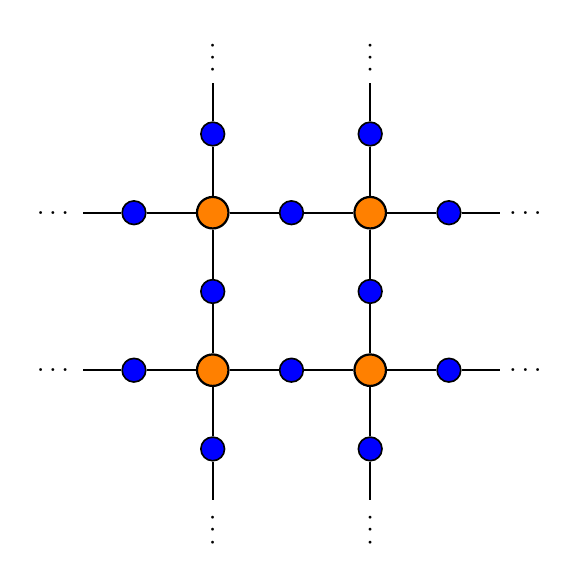
\begin{tikzpicture}
  \tikzstyle{tensor} = [circle, inner sep = 0pt, minimum size = 0.2cm]
  \tikzstyle{QTensor} = [tensor, semithick, draw, fill=blue, minimum size = 0.3cm]
  \tikzstyle{delta} = [tensor, thick, draw, fill=orange, minimum size = 0.4cm]
  \tikzstyle{ellipsisNode} = [tensor, minimum size = 0.7cm]

  % Draw delta tensors
  \foreach \x in {2, 4}
    \foreach \y in {2, 4}
      \node[delta] (\x-\y) at (\x, \y) {};

  % Draw Q tensors
  \foreach \x in {1, 3, 5}
    \foreach \y in {2, 4}
      {
      \node[QTensor] (\x-\y) at (\x, \y) {};
      \node[QTensor] (\y-\x) at (\y, \x) {};
      }

  % Draw ellipsis nodes
  \foreach \x in {0, 6}
    \foreach \y in {2, 4}
    {
    \node[ellipsisNode] (\x-\y) at (\x, \y) {$\dots$};
    \node[ellipsisNode, rotate = 90] (\y-\x) at (\y, \x) {$\dots$};
    }

  % Connections
  \foreach \x in {0, ..., 5}
    \foreach \y in {2, 4}
    {
    \pgfmathtruncatemacro{\neighbor}{\x + 1};
    \draw[thick] (\x-\y) -- (\neighbor-\y);
    \draw[thick] (\y-\x) -- (\y-\neighbor);
    }

\end{tikzpicture}
\end{document}
